\chapter{Testy oraz prezentacja wyników}
\label{cha: Tests}
Testy sprawdzające działanie aplikacji zostały przeprowadzone za pomocą komputera wyposażonego w czterordzeniowy procesor Intel\textregistered CORE\texttrademark i7 oraz pamięć RAM 16GB DDR3. 
W ramach testów wykorzystano bazę gestów opisaną w pracy \cite{Cambridge}. Zawiera ona 900 sekwencji obrazów tworząc 9 różnych klas. Klasy są utworzone na podstawie 3 prostych gestów dłoni, która jest poddawana rotacji. Każda z~klas zawiera 100 sekwencji obrazów (5 odmiennych warunków oświetleniowych, 10 różnych sekwencji ruchu dłoni w dwóch kierunkach). Każdy z gestów jest umieszczony na ciemnym tle bez dodatkowych elementów. Przykładowy zbiór obrazów reprezentujący gest dla różnych warunków oświetleniowych oraz rotacji zaprezentowano na rysunku \ref{im: Hands}.

\begin{figure}[h]
	%\centering
	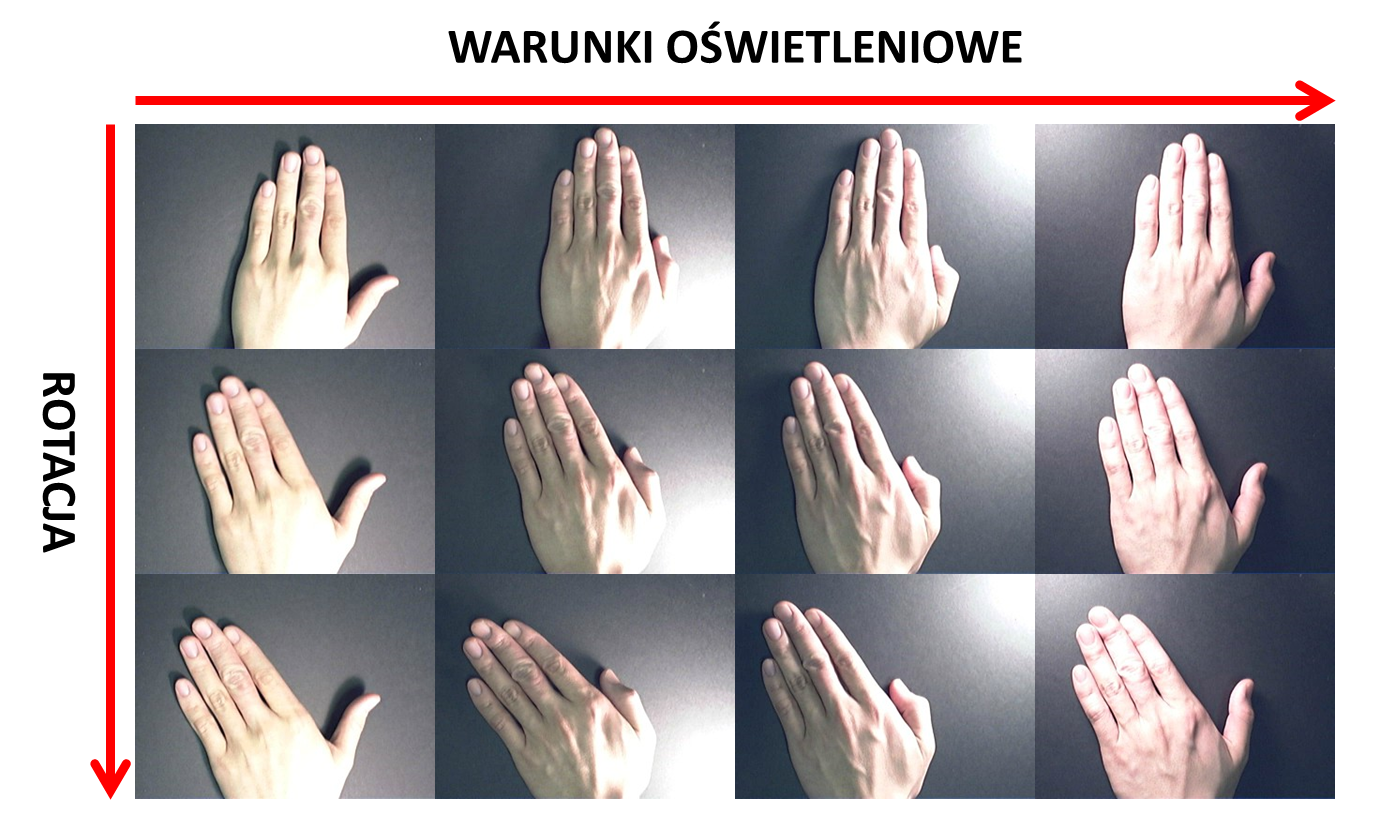
\includegraphics[width=15cm]{Hands}
	\centering
	\caption{Sekwencje gestów dostępne w bazie danych \cite{Cambridge}}
	\label{im: Hands}
\end{figure} 

Na potrzeby pracy z bazy wybrano 4 różne gesty, do których należały: dłoń ze złączonymi oraz rozłączonymi palcami (kolejno \textit{Palm} oraz \textit{Five Fingers}), pięść (\textit{Fist}) oraz dwa złączone palce (\textit{Two Fingers}).
Stworzono łącznie 33 sekwencje testowe. Różnią się one względem siebie wartościami poszczególnych parametrów. Pierwszy podział dotyczy ilości klastrów, na jakie podzielona została przestrzeń zmiennych opisujących cechy obrazu. Wybrano 3 wartości: 10, 36 oraz 50. Dla każdej z nich przeprowadzono następujące sekwencje testowe: 
\begin{enumerate}
	\item Wartość współczynnika funkcji kary: 100; Funkcja jądra: wielomianowa; Stopień wielomianu: 1; Stała wielomianu: 1; 
	\begin{enumerate}
		\item \label{tol1} Tolerancja: 0.00001
		\item \label{tol2} Tolerancja: 0.01
		\item \label{tol3} Tolerancja: 10
	\end{enumerate}
	\item Wartość współczynnika funkcji kary: 100; 
	Tolerancja: 0.00001; Funkcja jądra: wielomianowa;
	\begin{enumerate}
		\item \label{pol1} Stopień wielomianu: 1; Stała wielomianu: 1;
		\item \label{pol2}Stopień wielomianu: 1; Stała wielomianu: 50;
		\item \label{pol3} Stopień wielomianu: 1; Stała wielomianu: 1000;
		\item \label{pol4} Stopień wielomianu: 3; Stała wielomianu: 1;
		\item \label{pol5} Stopień wielomianu: 10; Stała wielomianu: 1;
	\end{enumerate}
	\item Wartość współczynnika funkcji kary: 100; 
	Tolerancja: 0.00001; Funkcja jądra: metoda RBF;
	\begin{enumerate}
		\item \label{sig1} Sigma: 10
		\item \label{sig2} Sigma: 20
		\item \label{sig3} Sigma: 5
	\end{enumerate}
\end{enumerate}

Dla każdego scenariusza zastosowano współczynnik określający skuteczność metody identyfikacji:
\begin{equation}
\textit{POPRAWNOŚĆ} = \frac{\textit{LICZBA PRÓBEK POPRAWNIE SKLASYFIKOWANYCH}}{\textit{LICZBA WSZYSTKICH PRÓBEK}} * \textit{100\%}
\end{equation}


\section{Wyniki testów dla próbek treningowych}
Z podanej bazy wybrano próbki stanowiące zestaw treningowy dla zaproponowanej metody identyfikacji gestów dłoni. Reprezentację każdego gestu stanowiło 360 obrazów zawierającą odmienne warunki oświetleniowe oraz różne pozycje podanego gestu. Całą bazę danych stanowiło 1440 obiektów. Wyniki testów dla deskryptora złożonego z 36 elementów przedstawiono w tabeli \ref{tab: train36}.

\begin{table} [h!]
	\centering
	\begin{tabular}{|c|c|c|c|c|c|}
		\hline
		\textbf{Sekwencja} 	& \textbf{Palm} & \textbf{Fist} & \textbf{Five Fingers} & \textbf{Two Fingers} & \textbf{Razem} \\ \hline
		\ref{tol1} 	& 88.6\% 		& 94.7\%		& 87.2\%	& 98.3\% 	& 92.2\% \\ \hline
		\ref{tol2} 	& 88.6\% 		& 94.7\%		& 87.2\%	& 98.3\% 	& 92.2\% \\ \hline
		\ref{tol3}	& 100\%			& 0\%			& 0\%		& 0\% 		& 25\% \\ \hline \hline
		\ref{pol1} 	& 88.6\% 		& 94.7\%		& 87.2\%	& 98.3\% 	& 92.2\% \\ \hline
		\ref{pol2} 	& 88.6\% 		& 94.4\%		& 86.9\%	& 99.2\% 	& 92.3\% \\ \hline
		\ref{pol3}	& 86.9\%		& 87.2\%		& 70.8\%	& 98.1\% 	& 89.4\% \\ \hline
		\ref{pol4}	& 86.9\%		& 98.1\%		& 86.7\%	& 96.7\% 	& 93.5\% \\ \hline
		\ref{pol5}	& 100\%			& 0\%			& 0\%		& 0\% 		& 25\% \\ \hline \hline
		\ref{sig1}	& 98.9\% 		& 98.9\%		& 98.6\%	& 99.7\% 	& 99.1\% \\ \hline
		\ref{sig2}	& 95.3\% 		& 95.6\%		& 92.8\%	& 99.4\% 	& 95.8\% \\ \hline
		\ref{sig3}	& 100\%			& 99.7\%		& 100\%		& 100\% 	& 99.9\% \\ \hline
	\end{tabular}
	\caption{Wyniki testów próbek treningowych dla deskryptora złożonego z 36 elementów.}
	\label{tab: train36}
\end{table}

Pierwsza sekcja to testy, w których zmieniano wartość tolerancji. Dla zbyt dużej wartości tego parametru klasyfikator był w stanie zaklasyfikować poprawnie tylko jeden gest. Zmiana parametru pomiędzy \textit{0.00001} a \textit{0.01} nie powodowała żadnych zmian w etapie klasyfikacji.    

Druga grupa testów to testy powiązane ze zmianą wartości współczynników dla wielomianowej funkcji jądra. Najlepszy rezultat osiągnięto dla wielomianu stopnia 3 oraz stałej równej 1. W przypadku, gdy stopień wynosił 10, klasyfikacja się nie powiodła. Zmiana wartości stałej wielomianu wnosiła nieznaczne wahania w kontekście poprawności klasyfikacji.

Najlepsze rezultaty osiągnięto w przypadku wykorzystania metody RBF jako funkcji jądra. Dokładność klasyfikacji wynosiła powyżej 95\% dla wszystkich przypadków. Scenariusz, w którym wartość parametru $\sigma$ wynosiła 5, skuteczność klasyfikacji była bliska 100\% - tylko jedna próbka została błędnie sklasyfikowana.

\begin{table} [h!]
	\centering
	\begin{tabular}{|c|c|c|c|c|c|}
		\hline
		\textbf{Sekwencja} 	& \textbf{Palm} & \textbf{Fist} & \textbf{Five Fingers} & \textbf{Two Fingers} & \textbf{Razem} \\ \hline
		\ref{tol1} 	& 81.9\% 		& 87.2\%		& 85\%		& 90.3\% 	& 86.1\% \\ \hline
		\ref{tol2} 	& 86.9\% 		& 86.4\%		& 84.4\%	& 90.1\% 	& 86\% \\ \hline
		\ref{tol3}	& 100\%			& 0\%			& 0\%		& 0\% 		& 25\% \\ \hline \hline
		\ref{pol1} 	& 81.9\% 		& 87.2\%		& 85\%		& 90.3\% 	& 86.1\% \\ \hline
		\ref{pol2} 	& 80.3\% 		& 86.4\%		& 82.2\%	& 92.5\% 	& 85.4\% \\ \hline
		\ref{pol3}	& 80.8\%		& 86.9\%		& 80.8\%	& 92.2\% 	& 85.2\% \\ \hline
		\ref{pol4}	& 81.1\%		& 88.9\%		& 80.3\%	& 85.6\% 	& 84\% \\ \hline
		\ref{pol5}	& 100\%			& 0\%			& 0\%		& 0\% 		& 25\% \\ \hline \hline
		\ref{sig1}	& 92.8\% 		& 90.6\%		& 94.7\%	& 99.2\% 	& 94.3\% \\ \hline
		\ref{sig2}	& 87.8\% 		& 87.8\%		& 86.7\%	& 96.4\% 	& 89.7\% \\ \hline
		\ref{sig3}	& 98.1\%		& 98.1\%		& 100\%		& 99.2\% 	& 98.8\% \\ \hline
	\end{tabular}
	\caption{Wyniki testów próbek treningowych dla deskryptora złożonego z 10 elementów.}
	\label{tab: train10}
\end{table}

Kolejny etap testów obejmował badanie poprawności klasyfikacji dla deskryptora złożonego z 10 elementów. Wyniki przedstawiono w tabeli \ref{tab: train10}.
Podobnie jak w przypadku deskryptora złożonego z 36 elementów najlepsze wyniki otrzymano dla scenariuszy wykorzystujących metodę RBF jako funkcję jądra. Jednakże każdy rezultat sprawdzający poprawność klasyfikacji był mniej dokładny niż dla przypadków opisanych w tabeli \ref{tab: train36}.

Ostatni zbiór scenariuszy testowych wykorzystujący próbki treningowe został przeprowadzony dla deskryptora złożonego z 50 elementów. Wyniki zawarto w tabeli \ref{tab: train50}.
\begin{table} [h!]
	\centering
	\begin{tabular}{|c|c|c|c|c|c|}
		\hline
		\textbf{Sekwencja} 	& \textbf{Palm} & \textbf{Fist} & \textbf{Five Fingers} & \textbf{Two Fingers} & \textbf{Razem} \\ \hline
		\ref{tol1} 	& 88.1\% 		& 95.6\%		& 90\%		& 99.4\% 	& 93.2\% \\ \hline
		\ref{tol2} 	& 87.5\% 		& 95.3\%		& 90.1\%	& 90.1\% 	& 99.7\% \\ \hline
		\ref{tol3}	& 100\%			& 0\%			& 0\%		& 0\% 		& 25\% \\ \hline \hline
		\ref{pol1} 	& 88.1\% 		& 95.6\%		& 90\%		& 99.4\% 	& 93.2\% \\ \hline
		\ref{pol2} 	& 88.1\% 		& 95\%			& 89.7\%	& 100\% 	& 93.2\% \\ \hline
		\ref{pol3}	& 87.2\%		& 90\%			& 84.2\%	& 95.3\% 	& 89.2\% \\ \hline
		\ref{pol4}	& 91.1\%		& 99.2\%		& 90\%		& 97.8\% 	& 94.5\% \\ \hline
		\ref{pol5}	& 100\%			& 0\%			& 0\%		& 0\% 		& 25\% \\ \hline \hline
		\ref{sig1}	& 99.4\% 		& 99.7\%		& 99.7\%	& 100\% 	& 99.7\% \\ \hline
		\ref{sig2}	& 93.3\% 		& 97.5\%		& 97.8\%	& 100\% 	& 97.2\% \\ \hline
		\ref{sig3}	& 100\%			& 100\%			& 100\%		& 100\% 	& 100\% \\ \hline
	\end{tabular}
	\caption{Wyniki testów próbek treningowych dla deskryptora złożonego z 50 elementów.}
	\label{tab: train50}
\end{table}
Podobnie jak dla dwóch powyższych przypadków, metoda RBF zwracała najbardziej zadowalające rezultaty. Dla sytuacji, w której wartość parametru $\sigma$ wynosiła 5 otrzymano 100\% poprawność klasyfikacji. 

W tabeli \ref{tab: train} zestawiono wynikowe rezultaty klasyfikacji dla każdego scenariusza testowego ze względu na liczbę klastrów. Najlepsze rezultaty otrzymano w przypadku deskryptora złożonego z 50 elementów. Wszystkie wyniki są lepsze od dwóch pozostałych przypadków (z wyłączeniem dwóch scenariuszy, w których klasyfikacja nie powiodła się). Najgorsze wyniki to rezultaty otrzymane dla deskryptora zbudowanego z 10 elementów. Wynika to z faktu, że wektor opisujący zbyt mocno generalizuje punkty kluczowe otrzymane z ekstrakcji cech za pomocą algorytmu SURF.  

\newpage

\begin{table} [h!]
	\centering
	\begin{tabular}{|c|c|c|c|}
		\hline
		\textbf{Sekwencja} 	& \textbf{36 klastrów} & \textbf{10 klastrów} & \textbf{50 klastrów} \\ \hline
		\ref{tol1} 	& 92.2\% 		& 86.1\%	& 93.2\% \\ \hline
		\ref{tol2} 	& 92.2\% 		& 86\%		& 99.7\% \\ \hline
		\ref{tol3}	& 25\%			& 25\%		& 25\%	 \\ \hline \hline
		\ref{pol1} 	& 92.2\% 		& 86.1\%	& 93.2\% \\ \hline
		\ref{pol2} 	& 92.3\% 		& 85.4\%	& 93.2\% \\ \hline
		\ref{pol3}	& 89.4\%		& 85.2\%	& 89.2\%	 \\ \hline
		\ref{pol4}	& 93.5\%		& 84\%		& 94.5\%	 \\ \hline
		\ref{pol5}	& 25\%			& 25\%		& 25\%	 \\ \hline \hline
		\ref{sig1}	& 99.1\% 		& 94.3\%	& 99.7\% \\ \hline
		\ref{sig2}	& 95.8\% 		& 89.7\%	& 97.2\% \\ \hline
		\ref{sig3}	& 99.9\%		& 98.8\%	& 100\%	 \\ \hline
	\end{tabular}
	\caption{Zestawienie wyników testów próbek treningowych ze względu na liczbę klastrów.}
	\label{tab: train}
\end{table}

\section{Wyniki dla próbek testowych}
Ostatni etap polegał na sprawdzaniu poprawności klasyfikacji próbek testowych. W tym celu wybrano nowe elementy z dostępnej bazy danych. Dla każdego gestu utworzono zestaw próbek składający się z 50 elementów. Wyniki dla odmiennych wartości parametrów umieszczono w tabelach. 

\begin{table} [h!]
	\centering
	\begin{tabular}{|c|c|c|c|c|c|}
		\hline
		\textbf{Sekwencja} 	& \textbf{Palm} & \textbf{Fist} & \textbf{Five Fingers} & \textbf{Two Fingers} & \textbf{Razem} \\ \hline
		\ref{tol1} 	& 61.4\% 	& 99.7\%	& 74.2\%	& 99.1\% 	& 83.6\% \\ \hline
		\ref{tol2} 	& 61.4\% 	& 99.4\%	& 74.2\%	& 99.4\% 	& 83.6\% \\ \hline
		\ref{tol3}	& -			& -			& -			& - 		& - 	 \\ \hline \hline
		\ref{pol1} 	& 61.4\% 	& 98.9\%	& 74.2\%	& 100\% 	& 83.6\% \\ \hline
		\ref{pol2} 	& 62.3\% 	& 98.5\%	& 73.8\%	& 98.1\% 	& 83.2\% \\ \hline
		\ref{pol3}	& 59.1\%	& 98.1\%	& 73.8\%	& 98.1\% 	& 82.3\% \\ \hline
		\ref{pol4}	& 55.7\%	& 97.4\%	& 75.4\%	& 96.2\% 	& 81.2\% \\ \hline
		\ref{pol5}	& -			& -			& -			& - 		& - 	 \\ \hline \hline
		\ref{sig1}	& 77.1\% 	& 98.5\%	& 76.9\%	& 98.3\% 	& 87.7\% \\ \hline
		\ref{sig2}	& 63.9\% 	& 97.7\%	& 70.7\%	& 98.8\% 	& 82.8\% \\ \hline
		\ref{sig3}	& 67.2\%	& 96.6\%	& 84.6\%	& 86.5\% 	& 83.7\% \\ \hline
	\end{tabular}
	\caption{Wyniki próbek testowych dla deskryptora złożonego z 36 elementów.}
	\label{tab: test36}
\end{table}

Pierwszy przypadek testowy dotyczył sytuacji, w której deskryptor był zbudowany z 36 elementów. Szczegóły w tabeli \ref{tab: test36}. Dla wszystkich scenariuszy testowych skuteczność klasyfikacji była wyższa niż 80\% Najlepszy rezultat otrzymano dla metody RBF jako funkcji jądra z parametrem $\sigma$ równym 10. Najwyższą skuteczność otrzymano dla gestu pięści - poprawność wyższa niż 90\%. Najgorzej wypadł gest dłoni - żaden rezultat nie przekroczył 80-cio procentowej poprawności klasyfikacji.  

Kolejny zestaw scenariuszy testowych wykonano dla deskryptora złożonego z 10 elementów. Wyniki przedstawiono w tabeli \ref{tab: test10}. Dla większości sytuacji poprawność klasyfikacja mieściła się pomiędzy 60 a 70\%. Dla przypadku, w którym wykorzystano metodę wielomianową stopnia 3 oraz dla stałej równej 1 otrzymano poprawność bliską 90\%. Najgorsze wyniki klasyfikacji wystąpiły dla gestu pięciu palców. Dla wielu przypadków poprawność wynosiła poniżej 30\%. 

\begin{table} [h!]
	\centering
	\begin{tabular}{|c|c|c|c|c|c|}
		\hline
		\textbf{Sekwencja} 	& \textbf{Palm} & \textbf{Fist} & \textbf{Five Fingers} & \textbf{Two Fingers} & \textbf{Razem} \\ \hline
		\ref{tol1} 	& 88.5\% 	& 99.5\%	& 27.7\%	& 50\% 		& 66.4\% \\ \hline
		\ref{tol2} 	& 86.9\% 	& 99.1\%	& 27.7\%	& 50\% 		& 65.9\% \\ \hline
		\ref{tol3}	& -			& -			& -			& - 		& - 	 \\ \hline \hline
		\ref{pol1} 	& 88.5\% 	& 99.5\%	& 27.7\%	& 50\% 		& 66.4\% \\ \hline
		\ref{pol2} 	& 86.9\% 	& 98.5\%	& 21.5\%	& 51.2\% 	& 64.5\% \\ \hline
		\ref{pol3}	& 86.9\%	& 98.5\%	& 21.5\%	& 55.8\% 	& 65.7\% \\ \hline
		\ref{pol4}	& 91.8\%	& 95.6\%	& 80.3\%	& 85.6\% 	& 88.3\% \\ \hline
		\ref{pol5}	& -			& -			& -			& - 		& - 	 \\ \hline \hline
		\ref{sig1}	& 80.3\% 	& 99.1\%	& 40.2\%	& 50\% 		& 67.4\% \\ \hline
		\ref{sig2}	& 77.1\% 	& 97.9\%	& 32.3\%	& 51.9\% 	& 64.8\% \\ \hline
		\ref{sig3}	& 83.6\%	& 93.2\%	& 53.9\%	& 46.2\% 	& 69.2\% \\ \hline
	\end{tabular}
	\caption{Wyniki próbek testowych dla deskryptora złożonego z 10 elementów.}
	\label{tab: test10}
\end{table}

Ostatni etap to testy dla deskryptora zbudowanego z 50-ciu elementów. Wyniki umieszczono w tabeli \ref{tab: test50}. Dla każdego scenariusza testowego rezultaty były wyższe niż 85\%. Najlepszą poprawność klasyfikacji  otrzymano dla metody wykorzystującą funkcję Gaussa z parametrem $\sigma$ równym 20. Skuteczność wynosiła 94\% - gesty pięści oraz dwóch palców zostały sklasyfikowane ze 100\% poprawnością. 

\begin{table} [h!]
	\centering
	\begin{tabular}{|c|c|c|c|c|c|}
		\hline
		\textbf{Sekwencja} 	& \textbf{Palm} & \textbf{Fist} & \textbf{Five Fingers} & \textbf{Two Fingers} & \textbf{Razem} \\ \hline
		\ref{tol1} 	& 88.5\% 	& 98.3\%	& 78.5\%	& 99.2\% 	& 91.1\% \\ \hline
		\ref{tol2} 	& 88.5\% 	& 98.3\%	& 78.5\%	& 99.2\% 	& 91.1\% \\ \hline
		\ref{tol3}	& -			& -			& -			& - 		& - 	 \\ \hline \hline
		\ref{pol1} 	& 88.5\% 	& 98.3\%	& 78.5\%	& 99.2\% 	& 91.1\% \\ \hline
		\ref{pol2} 	& 88.5\% 	& 98.5\%	& 78.5\%	& 97.3\% 	& 90.1\% \\ \hline
		\ref{pol3}	& 88.3\%	& 97.5\%	& 64.6\%	& 98.2\% 	& 87.2\% \\ \hline
		\ref{pol3}	& 80.3\%	& 97.5\%	& 84.6\%	& 94.2\% 	& 89.6\% \\ \hline
		\ref{pol5}	& -			& -			& -			& - 		& - 	 \\ \hline \hline
		\ref{sig1}	& 75.4\% 	& 98\%		& 95.4\%	& 100\% 	& 92.2\% \\ \hline
		\ref{sig2}	& 83.6\% 	& 100\%		& 92.3\%	& 100\% 	& 94\% \\ \hline
		\ref{sig3}	& 75.4\%	& 94.9\%	& 96.2\%	& 71.2\% 	& 84.4\% \\ \hline
	\end{tabular}
	\caption{Wyniki próbek testowych dla deskryptora złożonego z 50 elementów.}
	\label{tab: test50}
\end{table}


\newpage

\section{Podsumowanie testów}
W niniejszej sekcji zestawiono końcowe rezultaty klasyfikacji uwzględniając badany scenariusz, rodzaj próbek oraz długość wektora opisującego obraz. Szczegóły w tabeli \ref{tab: traintest}.
Najlepsza klasyfikacja uwzględniająca próbki treningowe oraz testowe wystąpiła dla metody wykorzystującej funkcję Gaussa przy parametrze $\sigma$ wynoszącym 20. Poprawność klasyfikacji dla obrazów treningowych wynosiła 97.2\%, natomiast dla próbek testowych 94\%. 

\begin{table} [h!]
	\centering
	\begin{tabular}{|c|c|c|c|c|c|c|}
		\hline
		\multirow{2}{*}{} & \multicolumn{3}{|c|}{Próbki Treningowe} & \multicolumn{3}{|c|}{Próbki Testowe} \\ \hline	
		& \textbf{36 klastrów} & \textbf{10 klastrów} & \textbf{50 klastrów} & \textbf{36 klastrów} & \textbf{10 klastrów} & \textbf{50 klastrów} \\ \hline
		
		\ref{tol1} 	& 92.2\% 	& 86.1\%	& 93.2\% 	& 83.6\%  	& 66.4\% 	& 91.1\% \\ \hline
		\ref{tol2} 	& 92.2\% 	& 86\%		& 99.7\% 	& 83.6\% 	& 65.9\% 	& 91.1\% \\ \hline
		\ref{tol3}	& 25\%		& 25\%		& 25\%	 	& - 		& - 		& - \\ \hline \hline
		\ref{pol1} 	& 92.2\% 	& 86.1\%	& 93.2\% 	& 83.6\% 	& 66.4\% 	& 91.1\% \\ \hline
		\ref{pol2} 	& 92.3\% 	& 85.4\%	& 93.2\% 	& 83.2\% 	& 64.5\% 	& 90.1\% \\ \hline
		\ref{pol3}	& 89.4\%	& 85.2\%	& 89.2\%	& 82.3\% 	& 65.7\% 	& 87.2\% \\ \hline
		\ref{pol4}	& 93.5\%	& 84\%		& 94.5\%	& 81.2\% 	& 88.3\% 	& 89.6\% \\ \hline
		\ref{pol5}	& 25\%		& 25\%		& 25\%		& -  		& - 		& - \\\hline \hline
		\ref{sig1}	& 99.1\% 	& 94.3\%	& 99.7\% 	& 87.7\% 	& 67.4\% 	& 92.2\% \\ \hline
		\ref{sig2}	& 95.8\% 	& 89.7\%	& 97.2\% 	& 82.8\% 	& 64.8\% 	& 94\% \\ \hline
		\ref{sig3}	& 99.9\%	& 98.8\%	& 100\%	 	& 83.7\% 	& 69.2\% 	& 84.4\% \\ \hline
	\end{tabular}
	\caption{Zestawienie końcowe próbek ze względu na liczbę klastrów.}
	\label{tab: traintest}
\end{table}
%Testy sprawdzające działanie aplikacji zostały przeprowadzone za pomocą komputera wyposażonego w czterordzeniowy procesor Intel\textregistered CORE\texttrademark i7 oraz pamięć RAM 16GB DDR3. W ramach testów wykorzystano ogólnie dostępne bazy danych zawierające gesty dłoni w zmieniających się warunkach oświetlenia. 
%Pierwszą z wykorzystanych baz była baza danych wykorzystana w pracy BIBLIOGRAFIA. Zawiera ona 900 sekwencji obrazów tworząc 9 różnych klas. Klasy te są utworzone na podstawie 3 prostych gestów dłoni, która jest poddawana rotacji oraz zaciskaniu w pięść. Szczegóły na rysunku RYSUNEK. Każda z klas zawiera 100 sekwencji obrazów (5 odmiennych warunków oświetleniowych, 10 różnych sekwencji ruchu dłoni w dwóch kierunkach). Każdy z gestów jest umieszczony na ciemnym tle bez dodatkowych elementów. 

%Na potrzeby pracy z bazy wybrano 5 różnych gestów, do których należały: dłoń ze (i) złączonymi oraz (ii) rozłączonymi palcami, (iii) pięść oraz dwa palce (iv) złączone oraz (v) rozłączone. 

%W ramach testów sprawdzono poprawność klasyfikacji gestu dla zmieniających się wartosci parametrów. Parametry poddane testom to: długość wektora opisującego gest, wybór metody \textit{kernel trick} (wraz z wpływem wartości poszczególnych parametrów), zmiany parametru funkcji kary oraz tolerancji.

%Dla każdego gestu 70\% wszystkich próbek zostało użyte w celu uczenia klasyfikatora, reszta to część testowa. 

%Dla każdego testu sprawdzono poprawność algorytmu rozpoznawania gestów dla część treningowej oraz testowej.  


%BOW = 36 Wielomianowa deg 1 con 1 compl= 1 tol = 1 czas wyliczenia poprawnosc testowa i treningowa

%BOW = 12 Wielomianowa deg 1 con 1 compl= 1 tol = 1 czas wyliczenie

%BOW = 72 Wielomianowa deg 1 con 1 compl= 1 tol = 1 czas wyliczenie

%BOW = 36 Gauss sigma = 1 compl= 1 tol = 1 czas wyliczenia

%BOW = 12 Gauss sigma = 1 compl= 1 tol = 1 czas wyliczenie

%BOW = 72 Gauss sigma = 1 compl= 1 tol = 1 czas wyliczenie

%Kolejna baza danych to zbiór obrazów dostępny 

%Ostatni etap to testowanie aplikacji wykorzystując urządzenie do rejestracji strumienia wideo. Do testów wykorzystano kamerę KAMERA operującą w rozdzielczości ROZDZIELCZOSC. 